\section{Energy Storage Sizing Approach} \label{sec:c4_approach}

As mentioned, previous IPS designs typically adopt a minimised capacitor size so as to minimise device dimensions and interruption periods, but this can also reduce forward progress.
An appropriate capacitor size instead may balance the three factors. 

We propose a sizing approach which recommends appropriate energy storage capacitance for an IPS, trading off forward progress against capacitor volume and interruption periods. 
We present a system model which accepts real long-term data on environmental energy conditions. 
The three inputs can be swept for design exploration, but we focus on energy storage in this chapter. 
The model outputs forward progress, capacitor volume, and interruption periods (defined in \sref{subsec:harvstor}). 
These are subsequently traded off in a cost function to obtain the appropriate energy storage capacitance. 
This process is summarised \fref{fig:sizingapproach} with details explained as follows. 

\begin{figure}
    \centering
    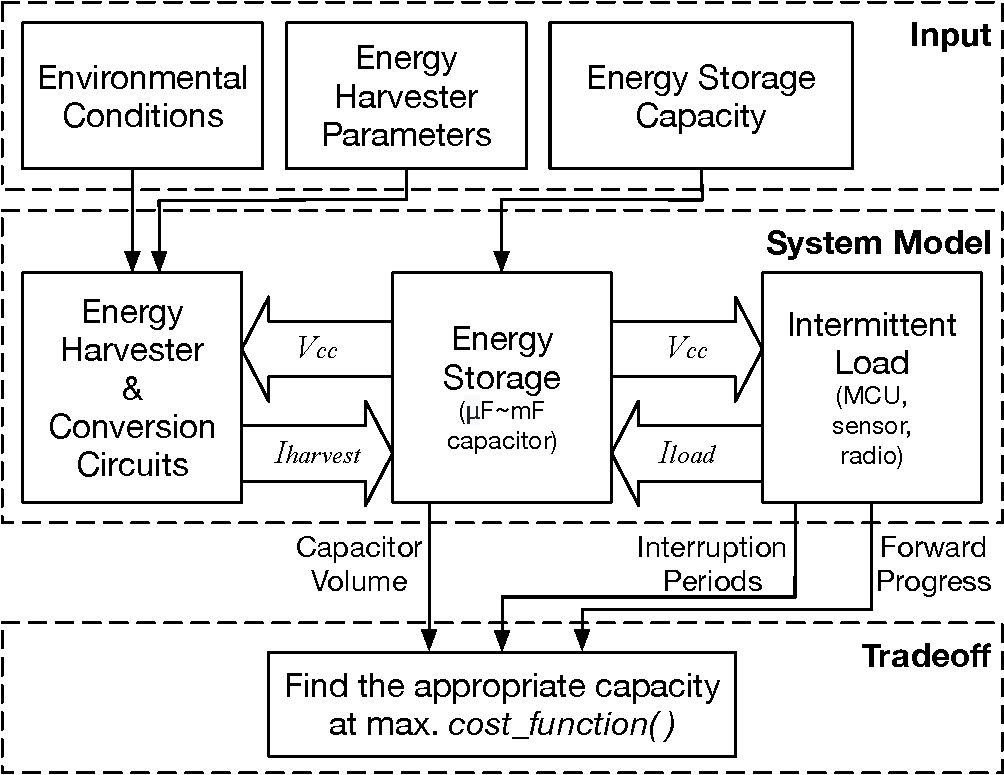
\includegraphics[width=\columnwidth]{ch4_sizingapproach/figures/mdlfrw5}
    \caption{Structure of the proposed system model and sizing approach.}
    \label{fig:sizingapproach}
\end{figure}
    
\subsection{Input}
A time trace of representative environmental energy conditions in the intended deployment location is provided as an input, along with the energy harvester size. 
For design exploration, assuming the energy source is equally distributed in the deployed space, these can optionally be changed to explore variations and scales of harvested power. 
A pre-defined set of energy storage capacitance values are swept through. 

\subsection{System Model}

This contains three modules, i.e. \textit{Energy Harvester and Conversion Circuits}, \textit{Energy Storage}, and \textit{Intermittent Load}. 
The three modules communicate by their voltage and current flows.
The current production \nm{I}{harv} and consumption \nm{I}{load} are buffered in the energy storage, which then calculates \nm{V}{cc} for the load and the harvester output. 
Due to the variety in each module, they should be individually specified to represent the target platform according to the techniques implemented. 

\begin{itemize}
    \item \textit{Energy Harvester and Conversion Circuits:} The energy harvester module transduces environmental energy into electricity. 
    The harvested power is typically conditioned to provide a suitable voltage for charging the energy storage and supplying the load efficiently. 
    In IPSs, conversion circuits may simply be a diode to inhibit backflow of current.
    The energy harvester and conversion circuits can be modelled together as a module because they are usually coupled or integrated. 
    \item \textit{Energy Storage:} Energy storage in IPSs is usually in the form of a \SI{}{\micro\farad}-  to \SI{}{\milli\farad}-scale capacitor. 
    It must be sufficient to complete the most energy-expensive atomic operation, and may be formed only of the decoupling capacitor(s). 
    This also includes an empirical model relating capacitance to capacitor volume (discussed in \sref{subsec:tradeoff}).
    %provides a minimum energy pulse, which should be set enough
    \item \textit{Intermittent Load:} It includes all the power consumers in an IPS, such as a microcontroller, sensors, and a radio. 
    This module outputs forward progress and interruption periods using the model presented in \sref{sec:c3_model}.
\end{itemize}

% As mentioned, IPS approaches can be classified as static and reactive approaches. These two types of approaches fundamentally differs in how the load consumes power and makes forward progress, and hence require different models for estimating forward progress. Owing to the computing advantage of reactive IPSs as explained in \sref{section:review}, we focus on reactive IPSs for modelling and validation in this paper.
% The unit of energy source conditions should be consistent with the unit of the \textit{Energy Harvester and Conversion Circuits} in the IPS model. 
% Note that the size configuration of energy harvester configures actual dimensions, e.g. PV panel area, while the one of energy storage configures capacitance.
% The size configuration of energy harvester and energy storage can be altered to observe how the design metrics change. 

\subsection{Trade-off}

The appropriate capacitance is then found through a cost function (an example of which is presented in \sref{subsec:tradeoff}). 
This may trade-off forward progress against capacitor volume and interruption periods.

% \footnote{Here, source power denotes the ambient energy source power exposed to energy harvester in a unit of the energy harvester model input. For example, if the energy harvester model is a photovoltaic (PV) cell model which takes irradiance as input, the source power should be defined in the unit of $W/m^2$. }

% Users should input a source power trace as a representation of the energy source conditions at the deployed site, and then alter the sizes of energy harvester and energy storage to explore the sizing effect on the design specifications. 

% For example, solar power from a solar panel is typically paired with a maximum power point tracking circuit to effectively extract solar power. The model should be configured for the specific energy harvester and the corresponding conversion circuits. 

% Static intermittent computing saves state at pre-installed points, and keeps executing until the supply fails, where the unsaved volatile progress is lost and the device has to re-execute from the last saved point. Reactive intermittent computing only saves state when the supply is about to fail (e.g. when the supply voltage is lower than a threshold), and then enters LPM (stop executing and enter a low-power mode). 
% However, to model intermittent computing is still a challenge due to lack of understanding and abstraction of its behaviours. 
% What is the difference of power consumption between these techniques? Power consumption: computing (CPU), memory R/W, peripherals (radio, ADC, sensor). While peripherals are more application-wise and currently we are not considering this, we focus more on memory R/W and CPU power. Memory R/W is related to both app and int techniques. Computing power, Memory R/W power. 